\section{Holland kippt} \footnote{Holland kippt Quelle: \cite{meeresspiegel2}}
1 zu 1:\newline
Der Abstand zwischen Meeresspiegel und Meeresboden an der niederländischen Küste wird nicht 
nur durch den Meeresspiegelanstieg größer, sondern auch durch das Absinken des Meeresbodens. 
Rijkswaterstaat rechnet mit einer Absenkung des Bodens im niedrigen nordwestlichen Teil der Niederlande 
bis 2100 zwischen 0.5 und 2 Meter, der hohe südöstliche Teil wird einige Zentimeter steigen. 
Die Niederlande kippen somit langsam aber stetig in Richtung Nordsee. Diese natürliche Bodenbewegung 
ist im vergangenen Jahrhundert gleichmäßig verlaufen.
\newline
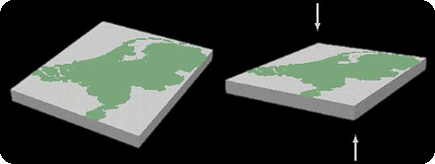
\includegraphics[width=1\textwidth]{images/niederlande_kippen.png}
\cite{kippen_bild} \text{Schema des Kippvorganges der Erdscholle}  
